\section{Numerical implementation and GPU execution}
\subsection{Time stepping and event accuracy}

The particle solver uses fixed-size arrays, release/activity masks, and a compiled integration loop. At each step it updates mass, evaluates forces, advances velocity, then advances position using the updated velocity:
\begin{equation}
 \vect v^{n+1}=\vect v^n+\Delta t\,\vect a^n,\qquad
 \vect r^{n+1}=\vect r^n+\Delta t\,\vect v^{n+1}.
\end{equation}
This is a first-order velocity-first Euler update, not a high-order CFD integration scheme. Sequential releases are quantized to $\operatorname{round}(t_{\mathrm{release}}/\Delta t)$. Native landing is recorded at the first step beyond the substrate plane; gutter reporting interpolates the crossing. Consequently step-size sensitivity is especially important for arrival-time and sub-10-micrometer placement claims. The substrate travels $v_s\Delta t$ per integration step, so time-step selection also sets a spatial event-resolution scale.

The native output includes positions, velocities, mass, radius, charge, individual force terms, directed Coulomb and wake labels, activity and lineage. Dense pair arrays scale as $O(P^2)$ per step for $P$ allocated particles. Recording all pair labels for all steps can dominate memory; capture intervals and event masks must be reported when comparing runtime.

The implementation uses JAX for compilation and accelerator execution \citep{jax,jaxjit}. The inverse-design procedure uses finite-difference sensitivities. Contact switches, nearest-neighbor selection, charge thresholds, release quantization, and substrate crossing make a blanket claim of a smooth, end-to-end differentiable raster optimizer inappropriate.


\subsection{Regular state and masked event handling}
Each simulation uses allocated arrays for position, velocity, mass, radius, charge, release time, and event state. A release mask selects emitted particles and an activity mask selects those still in flight. Unreleased, collected, deposited, or merged particles remain represented by masked array entries. This avoids dynamically resizing the particle set during compiled integration.

At each step, the operations are: update particle properties; interpolate the external field; evaluate pairwise separations and electric forces; determine eligible wake sources; evaluate carrier velocity and drag; advance state; and apply event rules. The reference implementation uses dense pair arrays, giving $O(P^2)$ pair work per step. GPU execution parallelizes this work; it does not change the quadratic asymptotic complexity.

\subsection{JIT compilation as an enabler, not the scientific contribution}
The implementation expresses the time integrator as a JIT-compiled scan. JAX traces the array program and lowers eligible operations to compiled accelerator execution \citep{jax,jaxjit}. Moving the repeated force and state-update sequence out of an interpreted loop reduces orchestration overhead and exposes parallel array operations to the compiler. The methodological contribution is independent of this specific compiler: it is the regular state and field--interaction decomposition that makes the formulation suitable for such execution.

Compilation is specialized to array shapes, types, static settings, and program structure. A changed particle capacity, step count, or static branch can require a new executable. Reuse depends on how the simulation callable and its inputs are organized; one must not assume that every new structural candidate shares an already compiled kernel. The current implementation is GPU-capable, while several archived search campaigns were executed on CPU. The new synchronized matched-workload benchmarks in Sec.~\ref{sec:framework_evidence} measure CPU/GPU performance separately from the archived searches.

\subsection{Performance accounting and memory}
For an inverse-design campaign, report
\begin{equation}
 T_{\mathrm{campaign}}=T_{\mathrm{field}}+T_{\mathrm{compile}}+
    \sum_{k=1}^K\left(T_{\mathrm{flight},k}+T_{\mathrm{transfer},k}
                           +T_{\mathrm{record},k}+T_{\mathrm{search},k}\right).
\end{equation}
Cold compilation, warmed execution, device transfers, and recording are different costs. Accelerator timings require synchronization at completion. Saving directed pair forces at every time step introduces $O(N_tP^2)$ output volume; this can dominate memory and transfer cost even when particle state is small. Sparse recording intervals, tiled pair evaluation, and neighbor lists are possible scalability extensions, but are not presumed to exist in the dense reference kernel.

A valid performance comparison uses identical force laws, particle counts, integration steps, event rules, and numerical precision. GPU acceleration must not be credited for changing the physical problem or omitting required output. No quantitative acceleration factor is inferred from the availability of JIT compilation alone.

\subsection{Reusable evaluation kernels and verification}
Dynamic charge vectors and contact-eligibility masks reuse one compiled executable at fixed capacity and physical configuration. Endpoint assessment retains landing, clearance and lineage diagnostics without materializing dense trajectories. A history-recording mode remains available for trajectory and force supervision. An inactive-state termination condition skips only post-flight steps after all particles are inactive. Reference-kernel tests check preserved full histories and event diagnostics; waveform response matrices are checked against the sequential charging routine.

\subsection{Euler--RK4 integration and timestep sensitivity}\label{sec:integration_comparison}
Both integrators use the same force evaluator and grid-boundary event policy. The Euler compatibility path retains the original mass-first, velocity-first update and passes preserved-solver parity checks. Classical RK4 advances $\vect y=(\vect r,\vect v,m)$ jointly, reevaluating the imposed field, pair forces, wake, drag and mass-loss rate at the four stages:
\begin{equation}
 \begin{aligned}
 \vect k_1&=F(\vect y_n,t_n), &\quad \vect k_2&=F(\vect y_n+\tfrac h2\vect k_1,t_n+\tfrac h2),\\
 \vect k_3&=F(\vect y_n+\tfrac h2\vect k_2,t_n+\tfrac h2), &\quad \vect k_4&=F(\vect y_n+h\vect k_3,t_n+h).
 \end{aligned}
\end{equation}
\begin{equation}
 \vect y_{n+1}^{\rm continuous}=\vect y_n+\frac h6(\vect k_1+2\vect k_2+2\vect k_3+\vect k_4).
\end{equation}
Release masks are held fixed during each step, then the same eligibility, greedy-contact, collection and first-crossing landing rules are applied. Detached charge is constant between events. The four-stage continuous method does not make discontinuous event handling fourth order.

For each case, the predeclared examples comprise an isolated least-deflected target, a complete stroke with blank history, two complete preceding/current strokes, and the worst context in the frozen full-pool reference. All use the same unchanged realized charges. Release times are rounded once to the native $1\,\mu$s schedule and held exactly fixed across integration refinements; otherwise changing release quantization would confound integration error. Euler and RK4 are evaluated at $h=1$, $0.5$ and $0.25\,\mu$s, with RK4 at $0.125\,\mu$s providing a finest numerical reference, not exact truth. Positive-air fluctuations are inactive in these cases. Native landing endpoints retain the original overshoot/event grid. Additional fixed-plane samples are linearly interpolated to distinguish trajectory differences from first-crossing endpoint quantization; samples spanning a merge are excluded with their denominators retained.

\begin{figure}[htbp]\centering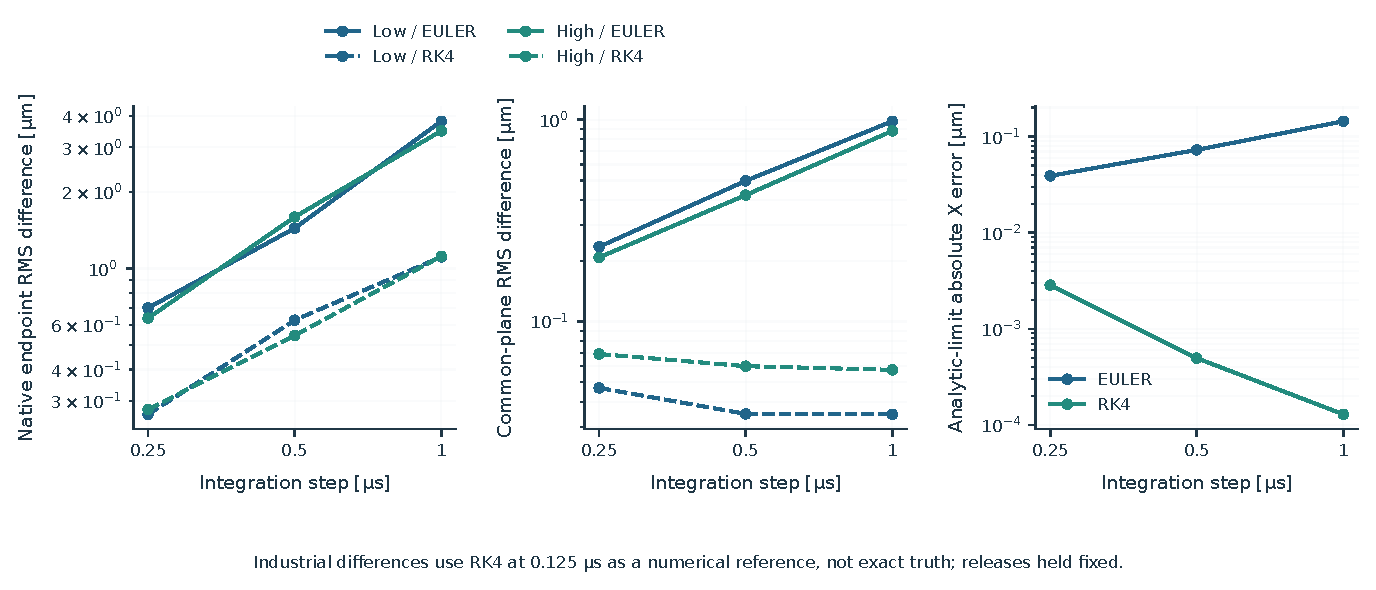
\includegraphics[width=\linewidth]{figures/integration_comparison.pdf}\caption{Numerical comparison at fixed release times and event rules. Left: native endpoint disagreement. Center: deflection disagreement at common axial planes. Both use the finest RK4 result as a numerical reference. Right: a separate event-free uniform-field/mass-loss limit has an analytic solution. Single precision and nonsmooth switching prevent assuming ideal asymptotic order for the complete industrial model.}\label{fig:integration_comparison}\end{figure}
For the low-speed examples at 1 microsecond, common-plane RMS deflection differences from the finest reference are 0.98 micrometers for Euler and 0.03 micrometers for RK4. For the high-speed examples at 1 microsecond, common-plane RMS deflection differences from the finest reference are 0.88 micrometers for Euler and 0.06 micrometers for RK4. All requested targets in these selected cases remain singleton landings, with no event-flag disagreements against the finest reference. Native endpoint RMS disagreements at 1 microsecond are approximately 3.5--3.8 micrometers for Euler and 1.1 micrometers for RK4; this distinction from common-plane errors reflects first-crossing overshoot. RK4 common-plane differences do not decrease monotonically at the finest steps, and the analytic-limit error also reaches a single-precision floor. These are numerical disagreements for selected trajectories, not errors against measured in-flight paths. The finest solution, event masks, interpolation and timestep remain part of the evidence boundary; a small optimized geometric residual does not certify equally small continuous-time error. The existing deposited-coordinate assessment retains its frozen native Euler reference and is not silently replaced by a newly optimized RK4 print.
\begin{figure}[htbp]\centering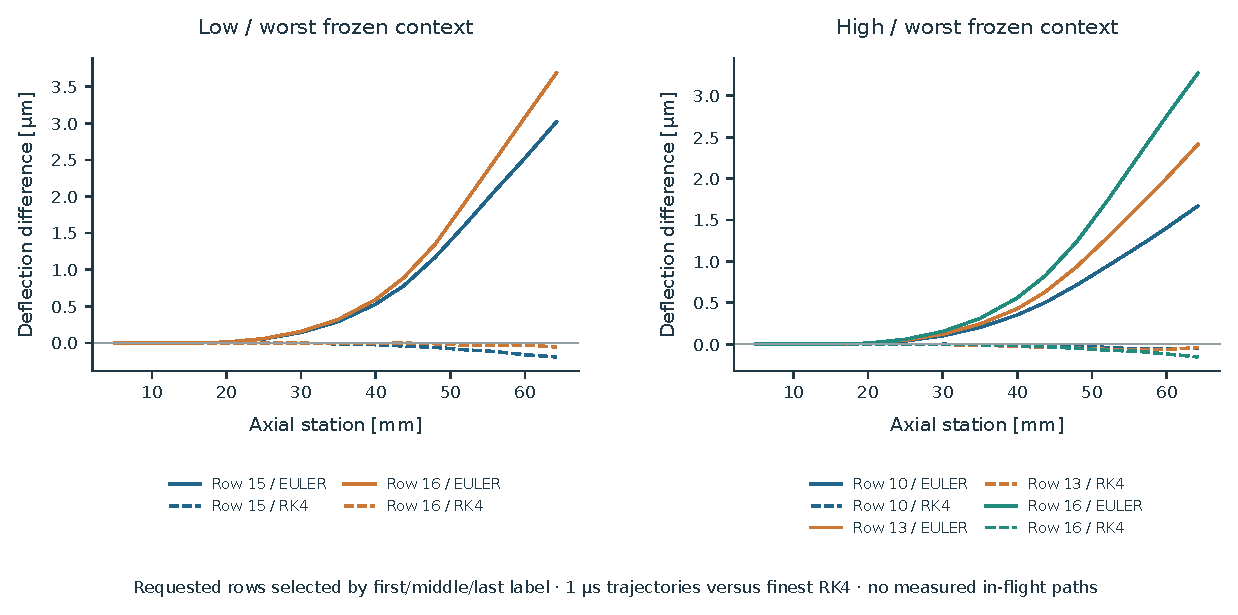
\includegraphics[width=\linewidth]{figures/integration_trajectory_differences.pdf}\caption{Representative trajectory differences at common axial stations for the worst preselected contexts. First/middle/last requested row labels are shown at the same integration step. This tests numerical integration, not experimental trajectory accuracy.}\label{fig:integration_trajectories}\end{figure}
